\documentclass[12pt,letterpaper]{article}
\usepackage{graphicx}
\usepackage{scrextend}
\usepackage{vmargin}
\usepackage{graphicx}
\usepackage{multirow}
\usepackage[utf8]{inputenc}
\usepackage[spanish]{babel}
\usepackage{multicol}
\usepackage{enumerate}
\usepackage{float}
\usepackage{amsmath, amsthm, amssymb, amsfonts}
\usepackage[usenames]{color}
\usepackage[breaklinks=true,hidelinks]{hyperref}
\parindent=0mm
\pagestyle{empty}
\definecolor{miorange}{rgb}{0.91, 0.43, 0.0}
\begin{document}
\setmargins{2.5cm}      
{1.5cm}                     
{2cm}  
{24cm}                    
{10pt}                          
{1cm}                          
{0pt}                             
{2cm}
\begin{titlepage}
\begin{center}

\includegraphics[scale=0.40]{../../../Logos/uanl.png} 
\hspace{2.5cm}

\includegraphics[scale=0.40]{../../../Logos/fcfm.png}
\end{center}
\vspace{2cm}
\begin{center}
\textbf{
UNIVERSIDAD AUTÓNOMA DE NUEVO LEÓN\\
FACULTAD DE CIENCIAS
FÍSICO MATEMÁTICAS}\\
\vspace*{2cm}
\begin{large}
\vspace{1cm}
\large{\textbf{Aplicaciones de la Mecánica Cuántica}}\\
\textbf{Radiación de cuerpo negro}\\
Carlos Luna Criado\\
\end{large}
\vspace{3.5cm}
\begin{minipage}{0.6\linewidth}
\vspace{0.5cm}
\changefontsizes{14pt}
Nombre:\\
Giovanni Gamaliel López Padilla\\
\end{minipage}
\begin{minipage}{0.2\linewidth}
\changefontsizes{14pt}
Matricula:\\
1837522
\end{minipage}
\end{center}
\vspace{4cm}
\begin{flushright}
\today
\end{flushright}
\end{titlepage}
\begin{multicols}{2}
\section*{Introducción}
A finales del siglo XIX y comienzos del siglo XX se desarrollaron avances científicos que influyeron en la teoría cuántica de la radiación del cuerpo negro, este problema en su época fue conocido como radiación negra \cite{Planck1901}. Si una cavidad de paredes perfectamente absorbentes se mantiene a una temperatura fija T, su interior contendra energía en forma de ondas. Si la radiación está en equilibrio, ya sea en su interior como en las paredes
, entonces la tasa con la que la energía es radiada a través de cualquier área unidad es independiente de la posición  orientación de dicha superficie. El determinar y explicar la forma de la intensidad de la radiación son las componentes principales del problema del cuerpo negro. \\
A principios del siglo XX, Rayleigh \cite{LordRayleigh1900} y Jeans \cite{JHJeans1902} realizaron cálculos de la densidad de energía de la irradiancia (radiación solar de un solo rango de longitutdes de onda) emitida por un cuerpo negro. Este resultado llevo a que las investigaciones hacia un conflicto entre los resultados experimentales y física clásica. Para encontrar alguna ley de distribución clasica, los dos autores tomaron como base a la teoría electromagnética clásica para demostrar la radiación dentro de la cavidad, en donde ellos proponian que esta debia de existir en frma de ondas estacionarias con nodos en las superficies dentro del cuerpo negro. De este modo, fue encontrada 
una ecuación para el número de ondas electromagnéticas estacionaras dentro del cuerpo, esta ecuación es la siguiente: 
\begin{equation}
    N(\nu)d\nu = \frac{8\pi V}{c^3} \nu^2 d\nu.
    \label{N(nu)dnu}
\end{equation}
En seguida, los autores realizaron el cálculo de la energía total promedio del sistema para cada onda con frecuencia $\nu$ utilizando la ley de equipartición de la energía, llegando a la ecuación
\begin{equation}
    \bar{E}=kT.
\end{equation}
Finalmente la irradiancia espectral clásica deducida por Rayleigh y Jeans es el producto del número de ondas estacionarias por unidad de volumen por la energía promedio y por la velocidad de la luz.
\begin{equation}
    R_T(\nu)d\nu = \frac{8\pi \nu^2 kT}{c^2} d\nu 
\end{equation}
dando así tambien la ecuación para la densidad de energía emitida por el cuerpo negro. 
\begin{equation}
    \rho_T(\nu) d\nu = \frac{8\pi \nu^2 k T}{c^3} d\nu 
\end{equation}
Al momento de comparar con los datos experimentales se percataron que para frecuencias altas (longitutdes de onda cortas) el espectro se iba hacia infinito, por lo que esto llevo a un problema, ya que esto no podia estar pasando. Esto se puede apreciar en la figura \ref{teovsexp}.
\begin{figure}[H]
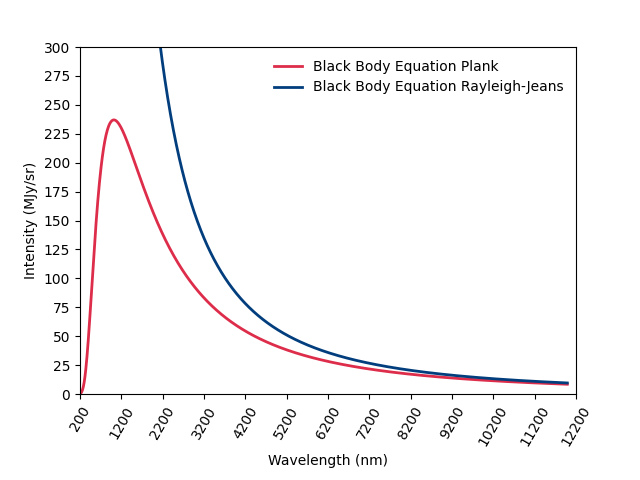
\includegraphics[scale=0.5]{../Graphics/exp_vs_teo.png}
\caption{Espectro de un cuerpo negro obtenido a partir de la ecuación de Plank y ecuación de Rayleigh-Jeans}
\label{teovsexp}
\end{figure}
\section*{Metodología}
\begin{equation}
S(\nu,T)= \frac{2h\nu^3}{c^2} \frac{1}{e^{h\nu/kT}-1}
\label{body equation}
\end{equation}
\section*{Resultados}
\begin{figure}[H]
    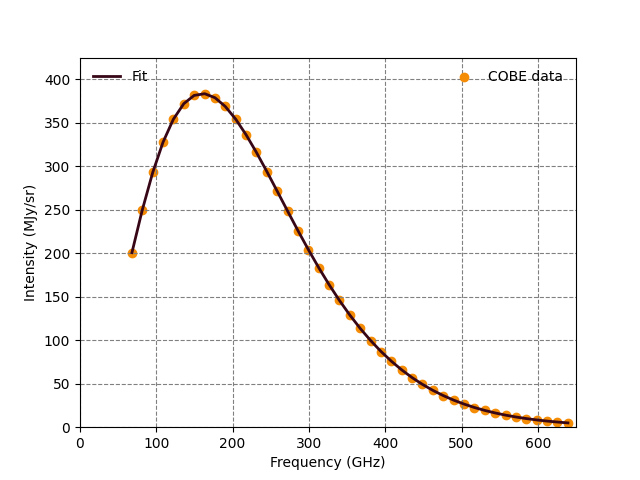
\includegraphics[scale=0.45]{../Graphics/fit.png}
    \caption{Fit de los datos proporcionados por el satelite FIRAS de la misión COBEA}
    \label{fit}
    \end{figure}
\begin{equation*}
    T=2.72502K
\end{equation*}
\begin{equation*}
    RD_i = \frac{|S_i(\nu,T)-COBE_i|}{COBE_i}*100\%
\end{equation*}
\begin{equation*}
    \langle RD \rangle = \sum\limits_{i=1}^N \frac{RD_i}{N} = 0.3205\%
\end{equation*}
\begin{equation*}
    R^2=0.99999972482939
    \label{coef_deter}
\end{equation*}
\begin{figure}[H]
    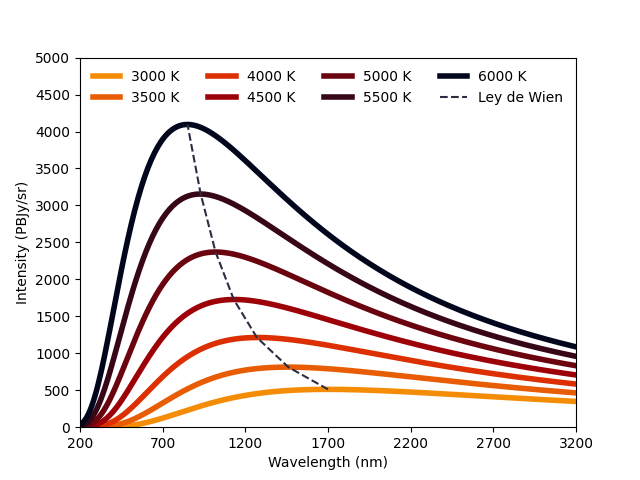
\includegraphics[scale=0.45]{../Graphics/black_body.png}
    \caption{Espectro electromagnetico para varias temperaturas.}
    \end{figure}
\section*{Conclusiones}
\bibliographystyle{plain}
\bibliography{Main}
\nocite{*}
\section*{Código}
\href{https://github.com/giovannilopez9808/Notas_Agosto_2020/blob/master/AMC/Reto1/black_body.py}{Github - black\_body.py}
\end{multicols}
\end{document}